\chapter{Efficiency of Sorting}
\label{CH:EFF:SORT}

Sorting rearranges input data according to a particular linear order
(see Section~\ref{sec:app:relations} for definitions of order and ordering 
relations). The most common examples are the usual dictionary (lexicographic) 
order on strings, and the usual order on integers.  

Once data is sorted, many other problems become easier to solve. Some of these 
include: finding an item, finding whether any duplicate items exist, finding the 
frequency of each distinct item, finding order statistics such as the maximum, 
minimum, median and quartiles. There are many other interesting applications of 
sorting, and many different sorting algorithms, each with their own strengths 
and weaknesses. In this chapter we describe and analyse some popular sorting 
algorithms.


\section{The problem of sorting}

The problem of sorting is to rearrange an input list of \defnfont{keys}, which 
can be compared using a total order $\leq$, into an output list such that if $i$
and $j$ are keys and $i$ precedes $j$ in the output list, then $i\leq j$.
Often the key is a data field in a larger object: for example, we may wish to 
sort database records of customers, with the key being their bank balance. 
If each object has a different key, then we can simply use the keys as identifiers
for the purpose of sorting: rather than moving large objects we need only keep 
a pointer from the key to the object. 

There are several important attributes of sorting algorithms.
\begin{Definition} 
A sorting algorithm is called \defnfont{comparison-based} if
the only way to gain information about the total order is by comparing a pair 
of elements at a time via the order $\leq$. 

A sorting algorithm is called \defnfont{stable} if whenever 
two objects have the same 
key in the input, they appear in the same order in the output. 

A sorting algorithm is called \defnfont{in-place} if it uses only a fixed 
additional amount of working space, independent of the input size.
\end{Definition}

With a comparison-based sorting algorithm, we cannot use any 
information about the keys themselves (such as the fact that they are all 
small integers, for example), only their order relation. These algorithms
are the most generally applicable and we shall focus exclusively 
on them in this book (but see Exercise~\ref{ex:radix}). 

We consider only two elementary 
operations: a \defnfont{comparison} of two items 
and a \defnfont{move} of an item. The running time of sorting algorithms in practice 
 is usually dominated by these operations. Every algorithm that we consider will make at 
most a constant number of moves for each comparison, so that the asymptotic 
running time in terms of elementary operations will be determined by the 
number of comparisons. However, lower order terms will depend on the exact number
of moves. Furthermore, the actual length of time taken by a data move depends 
on the implementation of the list. For example, moving an element from the 
end to the beginning of an array takes longer than doing the same for a linked 
list. We shall discuss these issues later.

The efficiency of a particular sorting algorithm may depend on many factors, 
for instance:

\begin{itemize}
\item how many items have to be sorted;
\item are the items only related by the order relation, or do they have other 
restrictions (for example, are they all integers from the range 1 to 1000);
\item to what extent they are pre-sorted;
\item can they be placed into an internal (fast) computer memory or must they be
sorted in external (slow) memory, such as on disk (so called 
\defnfont{external sorting}).
\end{itemize}

No one algorithm is the best for all possible situations, and so it is important
to understand the strengths and weaknesses of several algorithms.

As far as computer implementation is concerned, sorting makes sense only for 
linear data structures. We will consider lists (see Section~\ref{sec:app:adt-informal} 
for a review of basic concepts) which have a first element (the head), a last 
element (the tail) and a method of accessing the next element in constant time 
(an iterator). This includes array-based lists, and singly- and doubly-linked 
lists. For some applications we will need a method of accessing the previous 
element quickly; singly-linked lists do not provide this. Also, array-based 
lists allow fast random access. The element at any given position may be 
retrieved in constant time, whereas linked list structures do not allow this. 

\subsection*{Exercises}

\begin{Exercise}\label{exr:selection-sort-do} 
The  well-known and obvious \defnfont{selection sort} algorithm 
proceeds as follows.
We split the input list into a head and tail sublist. The head (``sorted") sublist is 
initially empty, and the tail (``unsorted") sublist is the whole list. 
The algorithm successively scans through the tail sublist to find the minimum 
element and moves it to the end of the head sublist. It terminates when the 
tail sublist becomes empty. (Java code for an array implementation is found 
in Section~\ref{sec:app:order}).

How many comparisons are required by selection sort in order to sort the input list 
$(6,4,2,5,3,1)$ ?  
\end{Exercise}

\begin{Exercise}\label{exr:selectionsort}
Show that selection sort uses the same number of comparisons on every input of 
a fixed size. How many does it use, exactly, for an input of size $n$? 
\end{Exercise}

\begin{Exercise}\label{exr:selsort-attributes}
Is selection sort comparison-based? in-place? stable?
\end{Exercise}

\begin{Exercise}\label{exr:find-duplicates}
Give a linear time algorithm to find whether a sorted list contains any 
duplicate elements. How would you do this if the list were not 
sorted?
\end{Exercise}

\section{Insertion sort}\label{sec:insort}

This is the method usually used by cardplayers to sort cards in their hand. 
Insertion sort is easy to implement, stable, in-place, and works well on small 
lists and lists that are close to sorted. However, it is very inefficient for 
large random lists.

Insertion sort is iterative and works as follows. The algorithm splits a list 
of size \(n\) into a head (``sorted") and tail (``unsorted") sublist.

\begin{itemize}
\item The head sublist is initially of size $1$. 
\item Repeat the following step until the tail sublist is empty:
\begin{itemize}
\item choose the first element $x$ in the tail sublist;
\item find the last element $y$ in the head sublist not exceeding $x$;
\item insert $x$ after $y$ in the head sublist.
\end{itemize}
\end{itemize}

Before each step $i=1, 2, \ldots, n-1$, the sorted and unsorted parts have $i$ 
and $n-i$ elements, respectively. The first element of the unsorted sublist is
moved to the correct position in the sorted sublist by exhaustive backward search,
by comparing it to each element in turn until the right place is reached. 

\begin{Example}
Table~\ref{t:is-example} shows the execution of insertion sort.
Variables $C_i$ and $M_i$ denote the number of comparisons and number of positions 
to move backward, respectively, at the $i$th iteration. Elements in the sorted 
part are italicized, the currently sorted element is underlined, and the element to 
sort next is boldfaced.
\end{Example}

\begin{table}[htb!]
\caption{Sample execution of insertion sort.}
\label{t:is-example}
\centerline{
  \begin{tabular}{|c|c|c|c|c|c|c|c|c|c|c|c|c|}
     \hline
$i$ & $C_i$ & $M_i$ & \multicolumn{10}{|c|}{\textbf{Data to sort}}\\
     \hline \multicolumn{3}{|c|}{} &
  \textit{25}&\textbf{8}&2& 91& 70& 50& 20& 31& 15& 65 \\ \hline  
1 & 1& 1& 
\underline{\textit{8}}&\textit{25}&\textbf{2}&91&70&50&20&31&15&65\\ \hline
2 & 2& 2& 
\underline{\textit{2}}&\textit{8}&\textit{25}&\textbf{91}&70&50&20&31&15&65\\ 
\hline
3 & 1& 0&\textit{2}&\textit{8}&\textit{25}& 
\underline{\textit{91}}&\textbf{70}&50&20&31&15&65\\ \hline
4 & 2& 1&\textit{2}&\textit{8}&\textit{25}& 
\underline{\textit{70}}&\textit{91}&\textbf{50}&20&31&15&65\\ \hline  
5 & 3& 2&\textit{2}&\textit{8}&\textit{25}& 
\underline{\textit{50}}& \textit{70}&\textit{91}&\textbf{20}&31&15&65\\ 
\hline  
6 & 5& 4&\textit{2}&\textit{8}& 
\underline{\textit{20}}& 
           \textit{25}& \textit{50}& \textit{70}&\textit{91}& 
           \textbf{31}&15&65\\ \hline  
7 & 4& 3&\textit{2}&\textit{8}& \textit{20}& \textit{25}& 
           \underline{\textit{31}}& \textit{50}& \textit{70}& 
           \textit{91}&\textbf{15}&65\\ \hline  
8 & 7& 6&\textit{2}&\textit{8}& \underline{\textit{15}}& \textit{20}&
           \textit{25}& \textit{31}&\textit{50}&\textit{70}&
           \textit{91}&\textbf{65}\\ \hline  
9 & 3& 2&\textit{2}& \textit{8}& \textit{15}& \textit{20}&\textit{25}& 
           \textit{31}&\textit{50}&\underline{\textit{65}}&
           \textit{70}&\textit{91}\\ \hline
 \end{tabular} } 
\end{table}

\subsection*{Analysis of insertion sort}

Insertion sort is easily seen to be correct (see Exercise~\ref{exr:isort2} for 
formal proof), since the head sublist is always sorted, and eventually expands to
include all elements.

It is not too hard to find the worst case for insertion sort: when the input 
consists of distinct items in reverse sorted order, every element must be 
compared with every element preceding it. The number of moves is also 
maximized by such input. The best case for insertion sort is when the input is 
already sorted, when only $n-1$ comparisons are needed.

%\newpage

\begin{Lemma} \label{lem:worst insort}
The worst-case time complexity of insertion sort is $\Theta(n^2)$.
\end{Lemma}
\begin{proof}
Fill in the details yourself --- see Exercise~\ref{exr:isort:max}.
\end{proof}

Since the best case is so much better than the worst, we might hope that on 
average, for random input, insertion sort would perform well. Unfortunately, 
this is not true.

\begin{Lemma}\label{lem:ave:insort}
The average-case time complexity of insertion sort is \(\Theta(n^2 )\).
\end{Lemma}

\begin{proof}
We first calculate the average number \(\overline{C_{i}}\) of comparisons
at the $i$th step. At the beginning of this step, $i$ elements of the head 
sublist are already sorted and the next element has to be inserted into the 
sorted part. This element will move backward $j$ steps, for some $j$ with 
$0 \leq j \leq i$. If $0 \leq j \leq i - 1$, the number of comparisons used will
be $j + 1$. But if $j=i$ (it ends up at the head of the list), there will be 
only $i$ comparisons (since no final comparison is needed).

Assuming all possible inputs are equally likely, the value of $j$ will be equally
likely to take any value $0, \dots, i$. Thus the expected number of comparisons 
will be 
$$
\overline{C_{i}} = \frac{1}{i+1} \left( 1 + 2 + \dots + i - 1 + i + i\right) 
 = \frac{1}{i+1} \left ( \frac{i(i+1)}{2}+i \right )
=  \frac{i}{2} + \frac{i}{i+1}.
$$
(see Section~\ref{sec:app:sum:series} for the simplification of the sum, if 
necessary).

The above procedure is performed for
$i=1,2, \ldots, n-1$, so that the average total number $\overline{C}$ of
comparisons is as follows: 
\begin{eqnarray*} \overline{C}
= \sum\limits_{i=1}^{n-1}\overline{C_{i}} = \sum\limits_{i=1}^{n-1}\left
(\frac{i}{2} + \frac{i}{i+1}\right) = \frac{1}{2}\sum\limits_{i=1}^{n-1}i
+ \sum\limits_{i=1}^{n-1}\frac{i}{i+1} 
\end{eqnarray*} 
The first sum is
equal to \(\frac{(n-1)n}{2}\).  To find the second sum, let us rewrite
\(\frac{i}{i+1}\) as \(1 - \frac{1}{i+1}\) so that 
\begin{eqnarray*}
\sum\limits_{i=1}^{n-1}\frac{i}{i+1} = \sum\limits_{i=1}^{n-1}\left (
1 - \frac{1}{i+1}\right ) = n-1 - \sum\limits_{i=1}^{n-1}\frac{1}{i+1} =
n - \sum\limits_{i=1}^{n}\frac{1}{i} = n - H_{n} 
\end{eqnarray*} 
where \(H_{n}\) denotes the \(n\)-th \defnfont{harmonic number}: 
\(H_{n}\approx \ln n \) when $n \rightarrow \infty$.

Therefore, $\overline{C} = \frac{(n-1)n}{4}+n - H_{n}$.
Now the total number of data moves is at least zero and at most the number 
of comparisons. Thus the total number of elementary operations is $\Theta(n^2)$.
\end{proof}

The running time of insertion sort is strongly related to \emph{inversions}. 
The number of inversions of a list is one measure of how far it is from being 
sorted.

\begin{Definition} 
An \defnfont{inversion} in a list $a$ is an ordered pair of positions 
$(i,j)$ such that $i<j$ but $a[i] > a[j]$. 
\end{Definition}

\begin{Example} The list $(3,2,5)$ has only one inversion corresponding to 
the pair $(3, 2)$, the list $(5,2,3)$ has two inversions, namely, $(5, 2)$ 
and $(5,3)$, the list $(3,2,5,1)$ has four inversions $(3,2)$, $(3,1)$, 
$(2,1)$, and $(5,1)$, and so on. 
\end{Example}

\begin{Example} 
Table~\ref{t:inversions} shows the number of inversions, $I_{i}$,
for each element $a[i]$ of the list in Table~\ref{t:is-example}
with respect to all preceding elements $a[0], \ldots, a[i-1]$
($C_i$ and $M_i$ are the same as in Table~\ref{t:is-example}).
\end{Example}

\begin{table}[htb!]
\caption[Number of inversions $I_i$, comparisons $C_i$ 
and data moves $M_i$.]%
{\label{t:inversions}Number of inversions $I_i$, comparisons $C_i$ 
and data moves $M_i$ for each element $a[i]$ in sample list.}
\centerline
{
\begin{tabular}{|c|c|c|c|c|c|c|c|c|c|c|}
\hline 
\textbf{Index} $i$     
& 0  & 1 & 2 & 3  & 4  & 5  & 6  & 7  & 8  & 9  \\ \hline
\textbf{List element} $a[i]$ 
& 25 & 8 & 2 & 91 & 70 & 50 & 20 & 31 & 15 & 65 \\ \hline
$I_{i}$ 
&    & 1 & 2 & 0  & 1  & 2  & 4  & 3  & 6  & 2 \\ %\hline 
$C_i$  
&    & 1 & 2 & 1  & 2  & 3  & 5  & 4  & 7  & 3 \\ %\hline 
$M_i$  
&    & 1 & 2 & 0  & 1  & 2  & 4  & 3  & 6  & 2 \\ \hline
\end{tabular}
}
\end{table}

Note that $I_i = M_i$ in Table~\ref{t:is-example}. This is not merely 
a coincidence---it is always true. See Exercise~\ref{exr:inversions}. 

The total number of inversions $I=\sum_{i=1}^{n-1}I_{i}$ in a list to be sorted 
by insertion sort is equal to the total number of positions an element moves 
backward during the sort. The total number of data comparisons 
$C=\sum_{i=1}^{n-1}C_{i}$ is also equal to the total number of inversions plus 
at most $n-1$. For the initial list in Tables~\ref{t:is-example} and 
\ref{t:inversions}, $I=21$, and insertion sort performs $C=28$ comparisons and 
$M=21$ data moves: in total, $49$ elementary operations.

Swapping two neighbours that are out of order removes exactly one inversion, 
and a sorted list has no inversions. If an original list has $I$ inversions, 
insertion sort has to swap $I$ pairs of neighbours. Because of $\Theta(n)$ 
other operations in the algorithm, its running time is $\Theta(n+I)$. 
Thus, on nearly sorted lists for which \(I\) is $\Theta(n)$, insertion sort 
runs in linear time. Unfortunately this type of list does not occur often, if 
we choose one randomly. As we have seen above, the average number of inversions 
for a randomly chosen list must be in $\Theta(n^2)$. This shows that more 
efficient sorting algorithms 
must eliminate more than just one inversion between neighbours per swap. One 
way to do this is a generalization of insertion sort called \emph{Shellsort}
(see Exercise~\ref{exr:shellsort}).

\subsection*{Implementation of insertion sort}

The number of comparisons does not depend on how the list is implemented, but 
the number of moves does. The insertion operation can be implemented in 
a linked list in constant time, but in an array there is no option but to shift 
elements to the right when inserting an element, taking linear time in the 
worst and average case. Thus if using an array 
implementation of a list, we may as well move the element backward by 
successive swaps. If using a linked list, we can make fewer swaps by simply 
scanning backward. On the other hand, scanning backward is easy 
in an array but takes more time in a singly linked list. However, none of 
these issues affect the asymptotic Big-Theta running time of the algorithm, 
just the hidden constants and lower order terms. The main problem with insertion
sort is that it takes too many comparisons in the worst case, no matter how 
cleverly we implement it.

Figure~\ref{f:is-sort2} shows basic pseudocode for arrays. 

\begin{figure}[htb!]
\hspace*{1in}\begin{minipage}{5in}
\Algorithm{insertionSort}
{array $a[0..n-1]$}
{the sorted array $a$}
{
\>\textbf{for} \(i \leftarrow 1\) \textbf{to} $n - 1$ \textbf{do}\\
\>\> \(k \leftarrow i-1\)\\
\>\> \textbf{while} \(k \ge 0 \) \textbf{and} 
 \(a[k] > a[k+1] \) \textbf{do}  \\
 \> \> \> \texttt{swap}($a,k,k+1$) \\
 \> \> \> \(k \leftarrow k-1\) \\
\>\>\textbf{end while} \\
\>\textbf{end for} \\
}
\end{minipage}
\caption{Insertion sort for arrays.}
\label{f:is-sort2}
\end{figure} 

\subsection*{Exercises}

\begin{Exercise}\label{exr:isort:inverse}
Determine the quantities $C_i$ and $M_i$ when insertion sort is run on the input
list \((91,70,65,50,31,25,20,15,8,2)\).  
\end{Exercise}

\begin{Exercise}\label{exr:isort2} Prove by induction that algorithm 
\algfont{insertionSort} is correct.
\end{Exercise}

\begin{Exercise}\label{exr:isort:max}
Prove that the worst-case time complexity of insertion sort is $\Theta(n^{2})$ 
and the best case is $\Theta(n)$.  
\end{Exercise}

\begin{Exercise}\label{exr:inversions}
Prove that the number of inversions, $I_{i}$, of an element \(a[i]\)
with respect to the preceding elements, \(a[0], \ldots, a[i-1]\), in the
initial list is equal to the number of positions moved backward by $a[i]$ 
in the execution of insertion sort.
\end{Exercise}  


\begin{Exercise}\label{exr:num:inversions} 
Suppose a sorting algorithm swaps elements  \(a[i]\) and 
\(a[i+ {\mathtt{gap}}]\) of a list \(a\) which were 
originally out of order.   
%\illustr{invers.eps}{80mm}        
Prove that the number of inversions in the list is reduced by at
least 1 and at most \(2 \ {\mathtt{gap}} - 1\).            
\end{Exercise}


\begin{Exercise}\label{exr:bubblesort} 
\defnfont{Bubble sort} works as follows to sort an array. There is a sorted 
left subarray and unsorted right subarray; the left subarray is initially empty. 
At each iteration we step through the right subarray, comparing each pair of 
neighbours in turn, and swapping them if they are out of order. At the end of 
each such pass, the sorted subarray has increased in size by 1, and we repeat 
the entire procedure from the beginning of the unsorted subarray. (Java code is 
found in Section~\ref{sec:app:order}.)

Prove that the average time complexity of bubble sort is $\Theta(n^{2})$, and 
that bubble sort never makes fewer comparisons than insertion sort.

\end{Exercise}

\begin{Exercise}\label{exr:shellsort}

\defnfont{Shellsort} is a generalization of insertion sort that works as follows. We first 
choose an \defnfont{increment sequence} $ \dots h_{t} > h_{t-1} > \ldots > h_{1}=1$. 
We start with some value of $t$ so that $h_t<n$. At each step we form the 
sublists of the input list $a$ consisting of elements $h:=h_t$ apart (for example, 
the first such list has the elements at position $0, h, 2h, \dots $, the next 
has the elements $1, 1+h, 1+2h, \dots $, etc). We sort each of these $h$ lists 
using insertion sort (we call this the \emph{$h$-sorting} step). We then reduce 
$t$ by $1$ and continue. Note that the last step is always a simple insertion 
sort.

Explain why Shellsort is not necessarily slower than insertion sort. Give an input 
on which Shellsort uses fewer comparions overall than insertion sort.
\end{Exercise}


\begin{Exercise}\label{exr:comparedata}
Find the total numbers of comparisons and backward moves performed by Shellsort on the 
input list \((91,70,65,50,31,25,20,15,8,2)\) and compare 
the total number of operations with that for insertion sort in 
Exercise~\ref{exr:isort:inverse}.
\end{Exercise}




\section{Mergesort}\label{sec:mergesort}

This algorithm exploits a recursive divide-and-conquer
approach resulting in a worst-case running time of $\Theta(n \log n)$, the 
best asymptotic behaviour that we have seen so far. Its best, worst, and average
cases are very similar, making it a very good choice if predictable runtime is 
important. Versions of mergesort are particularly good for sorting data with 
slow access times, such as data that cannot be held in internal memory or are 
stored in linked lists.
 
Mergesort is based on the following basic idea.
\begin{itemize}
\item If the size of the list is 0 or 1, return.
\item Otherwise, separate the list into two lists of equal or nearly equal size 
and recursively sort the first and second halves separately.
\item Finally, merge the two sorted halves into one sorted list.
\end{itemize}

Clearly, almost all the work is in the merge step, which we should make
as efficient as possible. Obviously any merge must take at least 
time that is linear in the total size of the two lists in the worst case, 
since every element must be looked at in order to determine the correct ordering.  
We can in fact achieve a linear time merge, as we see in the next section. 

\subsection*{Analysis of mergesort}

\begin{Lemma} Mergesort is correct.
\end{Lemma}
\begin{proof}
We use induction on the size $n$ of the list. If $n = 0$ or $1$, the result is 
obviously correct. Otherwise, mergesort calls itself recursively on two sublists
each of which has size less than $n$. By induction, these lists are correctly 
sorted. Provided that the merge step is correct, the top level call of 
mergesort then returns the correct answer. 
\end{proof}

Almost all the work occurs in the merge steps, so we need to perform those 
efficiently.

\begin{Theorem}
Two input sorted lists $A$ and $B$ of size $n_A$ and $n_B$, respectively, 
can be merged into an output sorted list $C$ of size $n_C = n_A + n_B$ in 
linear time.
\end{Theorem}

\begin{proof}
We first show that the number of comparisons needed is linear in $n$.
Let $i$, $j$, and $k$ be pointers to current positions in the lists
${A}$, ${B}$, and ${C}$, respectively. Initially,
the pointers are at the first positions, $i=0$, $j=0$, and $k=0$. Each
time the smaller of the two elements $A[i]$ and $B[j]$ is copied to
the current entry $C[k]$, and the corresponding pointers $k$ and either
$i$ or $j$ are incremented by 1. After one of the input lists is
exhausted, the rest of the other list is directly copied to
list ${C}$. Each comparison advances the pointer $k$ so that the
maximum number of comparisons is $n_A + n_B - 1$. 

All other operations also take linear time.
\end{proof}

The above proof can be visualized easily if we think of the lists as piles of 
playing cards placed face up. At each step, we choose the smaller of the two top
cards and move it to the temporary pile.


\begin{Example}
If $a=(2,8,25,70,91)$ and ${b}=(15,20,31,50,65)$, 
then merge into ${c}=(2,8,15,20,25,31,50,65,70,91)$ as follows.
\begin{description}
\item[Step 1] $a[0] =2$ and $b[0] =15$ are compared, $2 < 15$, and 
$2$ is copied to $c$, that is, $c[0] \leftarrow 2$, 
\(i\leftarrow 0+1\), and \(k\leftarrow 0+1\). 
\item[Step 2] $a[1] =8$ and $b[0] =15$ are compared to copy
$8$ to ${c}$, that is, $c[1] \leftarrow 8$,  
\(i\leftarrow 1+1\), and \(k\leftarrow 1+1\). 
\item[Step 3] $a[2] =25$ and $b[0] =15$ are compared 
and $15$ is copied to ${c}$ 
so that $c[2] \leftarrow 15$, \(j\leftarrow 0+1\), 
and \(k\leftarrow 2+1\).
\item[Step 4] $a[2] =25$ and $b[1] =20$ are compared and 
$20$ is copied to ${c}$: $c[3] \leftarrow 20$, \(j\leftarrow 1+1\), 
and \(k\leftarrow 3+1\). 
\item[Step 5] $a[2] =25$ and $b[2] =31$ are
compared, and $25$ is copied to ${c}$: $c[4] \leftarrow 25$, 
\(i\leftarrow 2+1\), and \(k\leftarrow 4+1\).
\end{description} 
The
process continues as follows: comparing $a[3] =70$ and $b[2] =31$,
$a[3] =70$ and $b[3] =50$, and $a[3] =70$ and $b[4] =65$
results in $c[5] \leftarrow (b[2] = 31)$, $c[6] \leftarrow(b[3] = 50)$, and
$c[7] \leftarrow(b[4] = 65)$, respectively. Because the list 
${b}$ is exhausted, the rest of the list $a$ is then copied to ${c}$,
$c[8] \leftarrow (a[3] =70)$ and $c[9]\leftarrow (a[4] =91)$.
\end{Example}

We can now see that the running time of mergesort is much better asymptotically 
than the naive algorithms that we have previously seen.

\begin{Theorem}
The running time of mergesort on an input list of size $n$ is $\Theta(n \log n)$ 
in the best, worst, and average case.
\end{Theorem}
\begin{proof}
The number of comparisons used by 
mergesort on an input of size $n$ satisfies a recurrence of the form 
\(T(n)=T(\lceil n/2\rceil )+ T(\lfloor n/2\rfloor ) + a(n)\) where 
$1\leq a(n)\leq n-1$. It is straightforward to show 
as in Example~\ref{exm:recur:d} that $T(n)$ is $\Theta(n \log n)$.

The other elementary operations in the divide and combine steps depend on the 
implementation of the list, but in each case their number is $\Theta(n)$. Thus 
these operations satisfy a similar recurrence and do not affect the 
$\Theta(n \log n)$ answer.
\end{proof}

\subsection*{Implementation of mergesort}

It is easier to implement the recursive version above for arrays than for 
linked  lists, since splitting an array in the middle is a constant time operation. 
Algorithm \algfont{merge} in Figure~\ref{merge} follows the above
description. The first half of the input array, \(a\), from the leftmost index 
$l$ to the middle index $m$ acts as $A$, the second half from $m + 1$ to the 
rightmost index $r$ as $B$, and a separate temporary array \({t}\) as ${C}$. 
After merging the halves, the temporary array is copied back to the original 
one, \(a\).

\begin{figure}[htb!]
\hspace*{.5in}\begin{minipage}{5in}
\Algorithm{mergeSort}
{
\begin{minipage}[t]{5in}
array $a[0..n-1]$; array indices $l, r$; array $t[0..n-1]$\\
\AlgCmt{sorts the subarray $a[l..r]$}
\end{minipage}
}
{the array $a$ with the sorted subarray $(a[l..r]$}
{
\> \textbf{if} $l < r$ \textbf{then} \\
\> \> $m \leftarrow \left \lfloor \frac{l+r}{2} \right \rfloor$\\
\> \>$\algfont{mergeSort}(a, l, m, t )$ \\
\> \>$\algfont{mergeSort}(a, m + 1,r, t )$ \\
\> \>$\algfont{merge}(a, l, m+1, r, t )$ \\
\> \textbf{end if}\\
}
\end{minipage}
\caption{\label{mergesort} Recursive mergesort for arrays}
\end{figure} 


\begin{figure}[htb!]
\hspace*{.5in}\begin{minipage}{5in}
\Algorithm{merge}
{
\begin{minipage}[t]{5in}
array $a[0..n-1]$; array indices $l, r$; array index $s$; array $t[0..n-1]$\\ 
\AlgCmt{merges the two sorted subarrays $a[l..s-1]$ and $a[s..r]$ into $a[l..r]$}
\end{minipage}
}
{the array $a$ with the sorted subarray $a[l..r]$ }
{
\> \(i\leftarrow l\); \(j \leftarrow s\); \(k\leftarrow l\)\\ 
\> \textbf{while} \(i \le s-1\) and \(j \le r\) 
                 \textbf{do}\\ % \hspace{10mm} \AlgCmt{main loop}\\
\> \>\textbf{if} \(a[i] \le a[j]\) \textbf{then} 
        \(t[k] \leftarrow a[i]\);
        \(k \leftarrow k + 1\); \(i \leftarrow i + 1\)\\
\> \>\textbf{else} \hspace{19mm}
        \(t[k] \leftarrow a[j]\);
        \(k \leftarrow k + 1\); \(j \leftarrow j + 1\)\\
\> \>\textbf{end if}\\
\> \textbf{end while} \\
\> \textbf{while} \(i \le s-1\) \textbf{do}
      \hspace{10mm}\AlgCmt{copy the rest of the first half}\\
\> \>\(t[k] \leftarrow a[i]\);
             \(k\leftarrow k + 1\); \(i\leftarrow i + 1\)\\
\> \textbf{end while} \\
\> \textbf{while} \(j \le r\) \textbf{do}
      \hspace{15mm}\AlgCmt{copy the rest of the second half}\\
\> \>\(t[k]\leftarrow a[j]\);
         \(k\leftarrow k + 1\); \(j\leftarrow j + 1\)\\
\> \textbf{end while} \\
\> \textbf{return} $a\gets t$ \\
} 
\end{minipage}
\caption{\label{merge} Linear time merge for arrays}
\end{figure} 


It is easy to see that the recursive version simply divides the list until it 
reaches lists of size $1$, then merges these repeatedly. We can eliminate the 
recursion in a straightforward manner. We first merge lists of 
size $1$ into lists of size $2$, then lists of size $2$ into lists of size $4$, 
and so on. This is often called \defnfont{straight mergesort}.

\begin{Example}\label{ex:straight-mergesort}
Starting with the input list $(1,5,7,3,6,4,2)$ we merge repeatedly. The merged
sublists are shown with parentheses. \\

\begin{tabular}{ll}
\begin{minipage}{2in}
Step~0: \ (1)(5)(7)(3)(6)(4)(2)\\
Step~1: \  (1,5)(3,7)(4, 6)(2)\\
\end{minipage} &
\begin{minipage}{2in}
Step~2: \ (1,3,5,7)(2,4,6)\\
Step~3: \ (1,2,3,4,5,6,7)\\
\end{minipage}
\end{tabular}
\end{Example}

This method works particularly well for linked lists, because the merge steps 
can be implemented simply by redefining pointers, without using the extra space 
required when using arrays (see Exercise~\ref{exr:linked-list-merge}). 

\subsection*{Exercises}

\begin{Exercise}\label{exr:mergesort-mincomp}
What is the minimum number of comparisons needed when merging two nonempty 
sorted lists of total size $n$ into a single list?
\end{Exercise}

\begin{Exercise}\label{exr:merge-hard-case}
Give two sorted lists of size $8$ whose merging requires the maximum number of 
comparisons.
\end{Exercise}

\begin{Exercise} \label{exr:insertion+merge}
The $2$-way merge in this section can be generalized easily to a $k$-way merge
for any positive integer $k$. The running time of such a merge is $c(k-1)n$. 
Assuming that the running time of insertion sort is $cn^{2}$ with the same 
scaling factor \(c\), analyse the asymptotic running time of the following 
sorting algorithm (you may assume that $n$ is an exact power of $k$).
\begin{itemize}
\setlength{\itemsep}{-3pt}
\item Split an initial list of size $n$ into $k$ sublists of size 
$\frac{n}{k}$ each. 
\item Sort each sublist separately by insertion sort.  
\item Merge the sorted sublists into a final sorted list. 
\end{itemize}
Find the optimum value of $k$ to get the fastest sort and compare its 
worst/average case asymptotic running time with that of insertion sort and 
mergesort.
\end{Exercise}

\begin{Exercise} \label{exr:linked-list-merge}
Explain how to merge two sorted linked lists in linear time into a bigger 
sorted linked list, using only a constant amount of extra space. 
\end{Exercise}


\section{Quicksort}\label{sec:qsort}

This algorithm is also based on the divide-and-conquer paradigm. Unlike 
mergesort, quicksort dynamically forms subarrays depending on the input,
rather than sorting and merging predetermined subarrays. Almost all the work of 
mergesort was in the combining of solutions to subproblems, whereas with 
quicksort, almost all the work is in the division into subproblems. 

Quicksort is very fast in practice on ``random" data and is widely used in 
software libraries. Unfortunately it is not suitable for mission-critical 
applications, because it has very bad worst case behaviour, and that behaviour 
can sometimes be triggered more often than an analysis based on random input 
would suggest.

Basic quicksort is recursive and consists of the following four steps. 

\begin{itemize}
\item  If the size of the list is 0 or 1, return the list. Otherwise:
\item Choose one of the items in the list as a \defnfont{pivot}. 
\item Next, \defnfont{partition} the remaining items into two disjoint sublists: 
reorder the list by placing all items greater than the pivot to follow it,
 and all elements less than the pivot to precede it.
\item Finally, return the result of quicksort of the ``head" sublist,
followed by the pivot, followed by the result of quicksort
of the ``tail" sublist.
\end{itemize}

The first step takes into account that recursive dynamic partitioning may produce 
empty or single-item sublists. The choice of a pivot at the next step is most 
critical because the wrong choice may lead to quadratic time complexity while a 
good choice of pivot equalizes both sublists in size (and leads to ``$n\log n$" 
time complexity). Note that we must specify
in any implementation what to do with items equal to the pivot. The third step is 
where the main work of the algorithm is done, and obviously we need to specify 
exactly how to achieve the partitioning step (we do this below). The final step
involves two recursive calls to the same algorithm, with smaller input.

\subsection*{Analysis of quicksort}

All analysis depends on assumptions about the pivot selection and partitioning 
methods used. In particular, in order to partition a list about a pivot element
as described above, we must compare each element of the list to the 
pivot, so at least $n-1$ comparisons are required. This is the right order: 
it turns out that there are several methods for partitioning that use 
$\Theta(n)$ comparisons (we shall see some of them below).

\begin{Lemma} 
Quicksort is correct.
\end{Lemma}
\begin{proof}
We use mathematical induction on the size of the list. If the size
is $1$, the algorithm is clearly correct. Suppose then that $n\geq 2$
and the algorithm works correctly on lists of size smaller than $n$. Suppose
that $a$ is a list of size $n$, $p$ is the pivot element, and $i$ is the
position of $p$ after partitioning. Due to the partitioning principle of 
quicksort, all elements of the head sublist are no greater than $p$, and all 
elements of the tail sublist are no smaller than $p$. By the induction hypothesis, 
the left and right sublists are sorted correctly, so that the whole list $a$
is sorted correctly.
\end{proof}

Unlike mergesort, quicksort does not perform well in the worst case.

\begin{Lemma}\label{lem:qsort:max} 
The worst-case time complexity of quicksort is \(\Omega(n^2 )\).
\end{Lemma}

\begin{proof}
The worst case for the number of comparisons is when the pivot is always the 
smallest or the largest element, one of two sublists is empty, and the second 
sublist contains all the elements other than the pivot. Then quicksort is 
recursively called only on this second group. We show that a quadratic number 
of comparisons are needed; considering data moves or swaps only increases the 
running time.

Let $T(n)$ denote the worst-case running time for sorting a list containing 
$n$ elements. The partitioning step needs (at least) $n-1$ comparisons. 
At each next step for $n \ge 1$, the number of comparisons is one less, so that
 \(T(n)\) satisfies the easy recurrence, 
\(T(n) = T(n-1) + n-1\); \(T(0)=0\), similar to the basic one, 
\(T(n)=T(n-1)+n\), in Example~\ref{exm:recur:a}. This yields that 
\(T(n)\) is $\Omega(n^{2})$. 
\end{proof}

However, quicksort is often used in practice, because it is fast on ``random" 
input. The proof of this involves a more complicated recurrence than we have 
seen so far.

\begin{Lemma}\label{lem:qsort:ave:comp}
The average-case time complexity of quicksort is \(\Theta(n\log n)\).
\end{Lemma}
\begin{proof}
Let $T(n)$ denote the average-case running time for sorting a list containing 
$n$ elements. In the first step, the time taken to compare all the elements with 
the pivot is linear, $cn$. If $i$ is the final position of the pivot,
then two sublists of size $i$ and $n-1-i$, respectively,
are quicksorted, and in this particular case \(T(n)=T(i)+T(n-1-i)+cn\). 
Therefore, the average running time to sort $n$ elements is equal to the
partitioning time plus the average time to sort $i$ and $n-1-i$ elements, where
$i$ varies from $0$ to $n-1$.

All the positions $i$ may be met \defnfont{equiprobably}---the pivot picked 
with the same chance \(\frac{1}{n}\)---as the final pivot position in a sorted
array.  Hence, the average time of each recursive call is equal to the 
average, over all possible subset sizes, of the average running time of 
recursive calls on sorting both subsets:
\begin{eqnarray*}
T(n) = \frac{1}{n} \sum\limits_{i=0}^{n-1} \left(T(i)+T(n-1-i)\right) +cn
= \frac{2}{n}\sum\limits_{i=0}^{n-1}T(i)+cn
\end{eqnarray*}
To solve this more difficult recurrence, let us rewrite it as
$$
nT(n)  = 2 \sum_{i=0}^{n-1}T(i) + cn^{2}
$$ 
and subtract the analogous one with $n$ replaced by $n-1$:
$$
(n-1)T(n-1)  = 2\sum_{i=0}^{n-2}T(i) + c(n-1)^{2}.
$$ 
After rearranging similar terms, we obtain
\(
%nT(n) = (n+1)T(n-1) + c\frac{2n+1}{n(n+1)}. 
nT(n)=(n+1)T(n-1)+c(2n-1) %Ulrich (22-May-12) 
\)
Decomposing the right side via partial fractions we obtain
$$
\frac{T(n)}{n+1} =
%\frac{T(n-1)}{n} + \frac{c}{n+1} + \frac{c}{n}. % Ulrich non-fix
\frac{T(n-1)}{n} + \frac{3c}{n+1} - \frac{c}{n}. % mjd June 2016 
$$
Telescoping of this recurrence results in the following relationship.
\begin{align*}
\frac{T(n)}{n+1} & = \frac{T(0)}{1}  +
%c\left (
%\frac{1}{2}+\frac{1}{3}+\frac{1}{4}+\ldots+\frac{1}{n+1} + 
3c\left (
\frac{1}{2}+\frac{1}{3}+\frac{1}{4}+\ldots+\frac{1}{n+1} 
\right ) - c\left (
\frac{1}{1} + \frac{1}{2}+\frac{1}{3}+\frac{1}{4}+\ldots+\frac{1}{n}
\right ) \\
& =  c (3H_{n+1}-3-H_{n})
 \end{align*}
where \(H_{n}\) is the $n$-th harmonic number.
Thus (see Section~\ref{sec:app:sum:series}) $T(n)$ is $\Theta(n \log n)$.
\end{proof}

This is the first example we have seen of an algorithm whose worst-case 
performance and average-case performance differ dramatically. 

The finer details of the performance of quicksort depend on several 
implementation issues, which we discuss next.

\subsection*{Implementation of quicksort}

There are many variants of the basic quicksort algorithm, and it makes sense to 
speak of ``a quicksort". There are several choices to be made:

\begin{itemize}
\item how to implement the list;
\item how to choose the pivot;
\item how to partition around the pivot.
\end{itemize}

\subsubsection*{Choosing a pivot}
A \defnfont{passive pivot strategy} of choosing 
a fixed (for example the first, last, or 
middle) position in each sublist as the pivot seems reasonable under the
assumption that all inputs are equiprobable. The simplest version of quicksort 
just chooses the first element of the list. We call this the \defnfont{naive 
pivot selection rule}.

For such a choice, the likelihood of a random input resulting in 
quadratic running time (see Lemma~\ref{lem:qsort:max} above) is very small. 
However, such a simple strategy is a bad idea. There are two main reasons:
\begin{itemize}
\item 
(nearly) sorted lists occur in practice rather frequently (think of a huge 
database with a relatively small number of updates daily);
\item 
a malicious adversary may exploit the pivot choice method by deliberately feeding
the algorithm an input designed to cause worst case behaviour (a so-called 
``algorithmic complexity attack").
\end{itemize}

If the input list is already sorted or reverse sorted, quadratic running time 
is obtained when actually quicksort ``should" do almost no work. We should look 
for a better method of pivot selection.

A more reasonable choice for the pivot is the middle element of each sublist. 
In this case an already sorted input list produces the perfect pivot at each 
recursion. Of course, it is still possible to construct  input sequences that 
result in quadratic running time for this strategy. They are very unlikely to 
occur at random, but this still leaves the door open for a malicious adversary. 

As an alternative to passive strategies, an \defnfont{active pivot strategy} 
makes good use of the input data to choose the pivot. The best active pivot is 
the exact median of the list because it partitions the list into (almost) 
equal sized sublists. But it turns out that the median cannot be computed 
quickly enough, and such a choice considerably slows quicksort down rather than 
improving it. Thus, we need a reasonably good yet computationally efficient 
estimate of the median. (See Section~\ref{sec:qselect} for more on the problem of 
exact computation of the  median of a list.)

A reasonable approximation to the true median is obtained by choosing the 
median of the first, middle, and last elements as the pivot 
(the so-called \defnfont{median-of-three} method). Note that this strategy is 
also the best for an already-sorted list because the median of each subarray 
is recursively used as the pivot.

\begin{Example}
\label{ex:qs-pivot}
Consider the input list of integers $(25, 8, 2, 91, 70, 50, 20, 31, 15, 65)$. Using the 
median-of-three rule (with the middle of a size $n$ list defined as the element 
at position $\lfloor n/2\rfloor$), the first pivot chosen is the median of 25, 
70 and 65, namely 65. Thus the left and right sublists after partitioning have 
sizes $7$ and $2$ respectively.

The standard choice for pivot would be the left element, namely $25$. In this 
case the left and right sublists after partitioning have sizes $4$ and $5$ 
respectively.
\end{Example}

The median-of-three  strategy does not completely avoid bad performance, 
but the chances of such a case occurring are much less than for a passive 
strategy. 

Finally, another simple method is to choose the pivot randomly. We can 
show (by the same calculation as for the average-case running time) 
that the expected running time on any given input is $\Theta(n \log n)$. It is 
still possible to encounter bad cases, but these now occur by bad luck, 
independent of the input. This makes it impossible for an adversary to force 
worst-case behaviour by choosing a nasty input in advance. 
Of course, in practice an extra overhead is incurred because of the work needed 
to generate a ``random" number. 

A similar idea is to first randomly shuffle the input (which can be done in 
linear time), and then use the naive pivot selection method. Again, bad cases 
still occur, but by bad luck only.

\subsubsection*{Partitioning}

There are several ways to partition with respect to the pivot element in linear 
time. We present one of them here. 

Our partitioning method uses a pointer $L$ starting at the head of the list
and another pointer $R$ starting at the end plus one. We first swap the pivot element to
the head of the list. Then, while $L < R$, we loop through the following procedure:

\begin{itemize}
\item Decrement $R$ until it meets an element less than or equal to $p$.
\item Increment $L$ until it meets an element greater than or equal to $p$.
\item Swap the elements pointed to by $L$ and $R$.
\end{itemize}
Finally, once $L = R$, we swap the pivot element with the element
pointed to by $L$.

\begin{Example}
\label{ex:qs-partition-example}
Table~\ref{qs-example} exemplifies the partitioning of a 10-element list. 
We choose the pivot $p=31$. The bold element is the pivot; elements in italics 
are those pointed to by the pointers $L$ and $R$.

\begin{table}[htb!]
  \caption{\label{qs-example}  Partitioning in quicksort with pivot $p=31$.}
\centerline{
{\small
\begin{tabular}{|c|c|c|c|c|c|c|c|c|c|l|}
     \hline
\multicolumn{10}{|c|}{\textbf{Data to sort}}& 
\textbf{Description} \\ \hline 
25 & 8 & 2 & 91 & 15 & 50 & 20 & 31 & 70 & 65    
& Initial list \\ \hline
\textbf{31}& 8 & 2 & 91 & 15 & 50 & 20 & 25 & 70 & 65    
& {Move pivot to head} \\ \hline  
\emph{\textbf{31}}& 8 & 2 & 91 & 15 & 50 & 20 & \emph{25} & 70 & 65 & stop $R$ \\ \hline
\textbf{31}& 8 & 2 & \emph{91} & 15 & 50 & 20 & 25 & 70 & 65 & stop $L$ \\ \hline
\textbf{31}& 8 & 2 &\emph{25}& 15 & 50 & 20 &\emph{91}& 70 & 65 & swap elements $L$ and $R$ \\ \hline 
\textbf{31}& 8 & 2 & \emph{25} & 15 & 50 & \emph{20} & 91 & 70 & 65 & stop $R$ \\ \hline 
\textbf{31}& 8 & 2 & 25 & 15 & \emph{50} & \emph{20} & 91 & 70 & 65 & stop $L$ \\ \hline
\textbf{31}& 8 & 2 & 25 & 15 &\emph{20} & \emph{50} & 91 & 70 & 65 & swap elements  $L$ and $R$ \\ \hline
\textbf{31}& 8 & 2 & 25 & 15 & \emph{20} & 50 & 91 & 70 & 65 & stop $R$ \\ \hline
20 & 8 & 2 & 25 & 15  &\textbf{\emph{31}} & 50 & 91 & 70 & 65 & swap element $L$ with pivot \\ \hline
\end{tabular}
}}
\end{table}

\end{Example}

\begin{Lemma}
The partitioning algorithm described above is correct.
\end{Lemma}
\begin{proof}
After each swap, we have the following properties: 
\begin{itemize}
\item each element to the left of $L$ (including the element at $L$) is less 
than or equal to $p$;
\item each element to the right of $R$ (including the element at $R$) is 
greater than or equal to $p$.
\end{itemize}
In the final swap, we swap the pivot element $p$ with an element that is no more 
than $p$. Thus all elements smaller than $p$ are now to its left, and all larger 
are to its right.
\end{proof}

We finish this section by discussing details associated with implementation of 
lists. Quicksort is much easier to program for arrays than for other types of 
lists. The pivot selection methods discussed above can be implemented in constant
time for arrays, but not for linked lists (for example, try the median-of-three 
rules with linked lists). The partition step can be performed on linked lists, 
but the method we have presented requires a doubly-linked list in order to work 
well, since we need to scan both forward and backward. 

In Figure~\ref{fig:quicksort} we present pseudocode for array-based quicksort. 
Here $i$ denotes the position of the pivot $p$ before the partition step, 
and $j$ its position after partitioning. The algorithm works in-place using the 
input array.

\begin{figure}[htb!]
\hspace*{.5in}\begin{minipage}{5in}
\Algorithm{quickSort}
{
\begin{minipage}[t]{5in}
array $a[0..n-1]$; array indices $l, r$\\
\AlgCmt{sorts the subarray $a[l..r]$}
\end{minipage}
}
{the list $a$ with the sorted subarray $(a[l..r]$}
{
\> \textbf{if} $l < r$ \textbf{then} \\
\> \> $i \leftarrow \algfont{pivot}(a,l,r)$ \AlgCmt{return position of pivot element}\\
\> \> $j \leftarrow \algfont{partition}(a,l,r,i)$ \AlgCmt{return final position of pivot}\\
\> \>$\algfont{quickSort}(a, l, j - 1)$  \AlgCmt{sort left subarray} \\
\> \>$\algfont{quickSort}(a, j+1, r)$   \AlgCmt{sort right subarray} \\
\> \textbf{end if}\\
\> \textbf{return} $a$\\
}
\end{minipage}
\caption{\label{fig:quicksort} Basic array-based quicksort.}
\end{figure} 

\subsection*{Exercises}

\begin{Exercise}\label{exr:qs-example}
Analyse in the same way as in Example~\ref{ex:qs-partition-example}
the next partitioning of the  left sublist 
$(20, 8, 2, 25, 15)$ obtained in Table~\ref{qs-example}.
\end{Exercise}

\begin{Exercise}\label{exr:qs-equal-keys-partition}
Show in detail what happens in the partitioning step if all keys are equal. 
What would happen if we change the partition subroutine so that 
$L$ skipped over keys equal to the pivot? What if $R$ did? 
What if both did? (hint: the algorithm would still be correct, but its performance 
would differ).
\end{Exercise}

\begin{Exercise}\label{exr:qs-bad:partition}
Analyse partitioning of the list
$(25, 8, 8, 8, 8, 8, 2)$ if the pointers $L$ and $R$ are advanced
while \(L \le p\) and \(p \le R\), respectively, rather than stopping on 
equality as in Table~\ref{qs-example}.
\end{Exercise}

\begin{Exercise} \label{exr:quicksort-extremes}
Suppose that we implement quicksort with the naive pivot choice rule and the 
partitioning method of the text. Find an array of size 8, containing each 
integer $1, \dots 8$ exactly once, that makes quicksort do the maximum number 
of comparisons. Find one that makes it do the minimum number of comparisons.
\end{Exercise}


\section{Heapsort}\label{sec:heapsort}

This algorithm is an improvement over selection sort that uses a more 
sophisticated data structure to allow faster selection of the minimum element. 
It, like mergesort, achieves $\Theta(n \log n)$ in the worst case. Nothing 
better can be achieved by an algorithm based on pairwise comparisons, as we 
shall see later, in Section~\ref{sec:lower:bound}.

A heap is a special type of tree. 
See Section~\ref{sec:app:trees} if necessary for general facts about trees.

\begin{Definition}
A \defnfont{complete binary tree} is a binary tree which is completely filled 
at all levels except, possibly, the bottom level, which is filled from left to
right with no missing nodes.
\end{Definition}

In such a tree, each leaf is of depth $h$ or $h-1$, where $h$ is the tree height, 
and each leaf of height $h$ is on the left of each leaf of height $h-1$.

\begin{Example} Figure~\ref{tree-fig} demonstrates a complete binary tree with 
ten nodes. If the node $J$ had been the right child of the node $E$, the
tree would have not been complete because of the left child node missed at the 
bottom level.
\end{Example}       
           
                                                
\begin{figure}[htb!]
\centerline{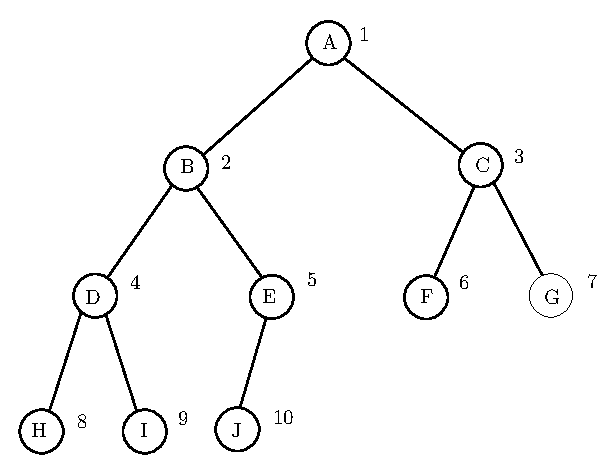
\includegraphics[width=80mm]{figs/tree-figTop.eps}}
\centerline{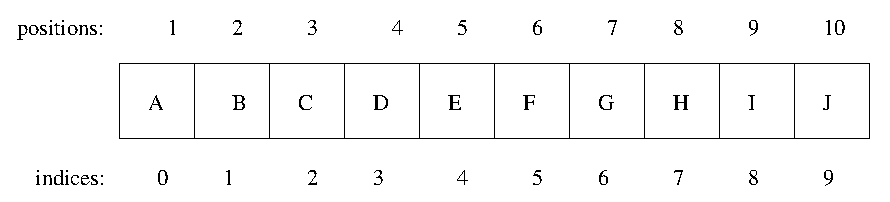
\includegraphics[width=80mm]{figs/tree-figBottom.eps}}
\caption{Complete binary tree and its array representation.}
\label{tree-fig} 
\end{figure}

A level-order traversal of a complete binary tree is easily stored
in a linear array as shown in Figure~\ref{tree-fig}. In this book 
we mostly use indices $0$ to $n-1$ for the array positions $1$ to $n$ 
in order to match popular programming languages such as Java, C, or C++. 
But the array representation of a binary tree is 
described more conveniently when both
the node numbers and the array positions are changing
from $1$ to $n$. Therefore, when a position $p$ in an array $a$
is mentioned below, we bear in mind 
an array element $a[i]$ with the index $i=p-1$.

The node in position $p$ has its parent node, left child, and right
child in positions $\lfloor p/2 \rfloor$, $2p$, and $2p + 1$,
respectively. The leaves have no children so that for each leaf node
$q$, the child position $2q$ exceeds the number of nodes $n$ in the
tree: $2q > n$.

\begin{Example}
In Figure~\ref{tree-fig},
the node in position $p=1$ is the root with no parent node. 
The nodes in positions from 6 to 10
are the leaves. The root has its
left child in position $2$ and its right child in position 
$3$. The nodes in positions $2$ and $3$ 
have their left child in position
$4$ and $6$ and their right child in position $5$ and $7$, respectively. 
The node in position $4$
has a left child in position $8$ and a right child in position
$9$, and the node $5$ has only a left child, in position $10$. 
\end{Example}

\begin{Definition}
A (maximum) \defnfont{heap} is a complete binary tree
having a key associated with each node,
the key of each parent node being greater than or
equal to the keys of its child nodes. 
\end{Definition} 

The heap order provides easy access to the maximum key  
associated with the root.

\begin{Example}
Figure~\ref{heap-fig} illustrates a maximum heap. Of
course, we could just as easily have a minimum heap  where
the key of the parent node is less than or equal to the keys
of its child nodes. Then the minimum key is associated with
the root. 
\end{Example}

\begin{figure}[htbp]
\begin{center}
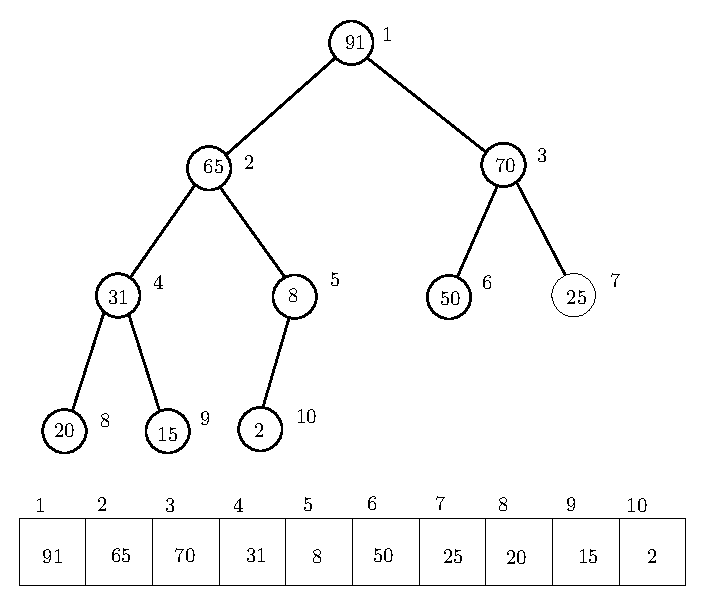
\includegraphics[width=80mm]{figs/heapmjd2ipe.eps}
\caption{\label{heap-fig} Maximum heap and its array representation.}
\end{center}
\end{figure}

The \defnfont{heapsort} algorithm now works as follows. Given an input list, 
build a heap by successively inserting the elements. Then delete the maximum 
repeatedly (arranging the elements in the output list in reverse order of 
deletion) until the heap is empty. Clearly, this is a variant of selection 
sort that uses a different data structure.

\subsection*{Analysis of heapsort}

Heapsort is clearly correct for the same reason as selection sort. To analyse its
performance, we need to analyse the running time of the insertion and deletion 
operations.

\begin{Lemma}\label{lem:tree:height}
The height of a complete binary tree with $n$ nodes
is at most $\lfloor \lg n \rfloor$.
\end{Lemma}

\begin{proof} Depending on the number of nodes at the bottom level,
a complete tree of height $h$ contains between $2^{h}$ and
$2^{h+1}-1$ nodes, so that \(2^{h} \le n < 2^{h+1}\),
or \(h \le \lg n < h+1\). \end{proof}


\begin{Lemma} 
Insertion of a new node into a heap takes logarithmic time. 
\end{Lemma}

\begin{proof}
To add one more node to a heap of \(n\) elements, a new,
\((n+1)\)-st, leaf position has to be created. The new node with 
its associated key is placed first in this leaf.  
If the inserted key preserves the heap order, the insertion is
completed. Otherwise, the new key has to swap with
its parent, and this process of \defnfont{bubbling up}, 
(or \emph{percolating up}) the key is repeated toward the root until the heap 
order is restored. Therefore, there are at most $h$ swaps where $h$ is the heap 
height, so that the running time is $O(\log n)$.
\end{proof}

\begin{Example}
To insert an 11th element, $75$, into the heap
in Figure~\ref{heap-fig} takes three steps.
\begin{itemize}
\item Position 11 to initially place the new key, $75$, is created.
\item The new key is swapped with its parent key, $8$, in
position $5 = \lfloor 11/2 \rfloor$ to restore the heap order.
\item The same type of swap is repeated for the parent key, $65$, 
in position $2 = \lfloor 5/2 \rfloor$. Because the heap order condition is now 
satisfied, the process terminates.
\end{itemize}

\begin{table}[htb!]
\caption{Inserting a new node with the key 75 in the heap 
in Figure~\ref{heap-fig}.}\label{t:insert:heap}
\centerline{
\begin{tabular}{|l|c|c|c|c|c|c|c|c|c|c|c|} \hline
\textbf{Position} & 1 & 2 & 3 & 4 & 5 & 6 & 7 & 8 & 9 & 10 & 11 \\ \hline 
\textbf{Index}   & 0 & 1 & 2 & 3 & 4 & 5 & 6 & 7 & 8 & 9 & 10 \\ \hline
Array at step 1 & 91 & 65 & 70 & 31 & 8 & 50 & 25 & 20 & 15 & 2 & \textbf{75} 
\\ %\hline
Array at step 2 & 91 & 65 & 70 & 31 & \textbf{75} & 50 & 25 & 20 & 15 & 2 & 
\emph{8} 
\\ %\hline
Array at step 3 & 91 & \textbf{75} & 70 & 31 & \emph{65} & 50 & 25 & 20 & 15 & 2 
& 8 
\\ \hline
\end{tabular}}
\end{table}

This is shown in Table~\ref{t:insert:heap}. The elements moved to
restore the heap order are italicized.

\end{Example}


\begin{Lemma} \label{lem:heap-delete}
Deletion of the maximum key from a heap takes logarithmic time in the worst case.
\end{Lemma}

\begin{proof}
The maximum key occupies the tree's root, that is, position 1 of the array.
The deletion reduces the heap size by 1 so that its last leaf node has to be 
eliminated. The key associated with this leaf replaces the deleted
key in the root and then is \defnfont{percolated down} the tree. 
First, the new root key is compared to each child and swapped with the larger 
child if at least one child is greater than the parent. This process is 
repeated until the order is restored. Therefore, there are $h$ moves in the 
worst case where $h$ is the heap height, and the running time is $O(\log n)$. 
\end{proof}

Because we percolate down the previous leaf key, the process usually
terminates at or near the leaves. 

%\newpage

\begin{Example}
To delete the maximum key, $91$, from the heap in Figure~\ref{heap-fig}, takes 
three steps, as follows.

\begin{itemize}
\item Key $2$ from the eliminated position 10 is placed at the root.
\item The new root key is compared to its children $65$ and $70$ in positions
 $2 = 2 \cdot 1 $  and $3 = 2 \cdot 1 + 1$, respectively. To restore 
the heap order, it is swapped with its larger child, $70$.
\item The same swap is repeated for the children $50$ and $25$ in 
positions $6 = 2 \cdot 3$ and $7 = 2 \cdot 3 + 1$. Because the heap order 
is now correct, the process terminates.
\end{itemize}

\begin{table}[htb!]
\caption{\label{t:delete:heap}
Deletion of the maximum key from the heap in Figure~\ref{heap-fig}.}
\centerline{
\begin{tabular}{|l|c|c|c|c|c|c|c|c|c|} \hline
\textbf{Position} & 1 & 2 & 3 & 4 & 5 & 6 & 7 & 8 & 9  \\ \hline
\textbf{Index}   & 0 & 1 & 2 & 3 & 4 & 5 & 6 & 7 & 8  \\ \hline
Array at step 1 & \textbf{ 2} & 65 & 70       & 31 & 8 & 50 & 25 & 20 & 15 
\\ %\hline
Array at step 2 & \emph{70} & 65 & \textbf{ 2} & 31 & 8 & 50 & 25 & 20 & 15  
\\ %\hline
Array at step 3 & \emph{70} & 65 & \emph{50} & 31 & 8 & \textbf{2} & 25 & 20 & 15 
\\ \hline
\end{tabular}}
\end{table}

See also Table~\ref{t:delete:heap}.
The leaf key replacing the root key is boldfaced, and the moves to restore the 
heap are italicized.

\end{Example}

\begin{Lemma}
Heapsort runs in time in $\Theta(n \log n)$ in the best, worst, and average case.
\end{Lemma}
\begin{proof}
The heap can be constructed in time $O(n \log n)$ (in fact it can be done more 
quickly as seen in Lemma~\ref{lem:quickheap} 
but this does not affect the result). Heapsort then repeats $n$ times the 
deletion of the maximum key and restoration of the heap property. 
In the best, worst,  and average case, each restoration is logarithmic, so the
 total time is $\log(n)+\log(n-1)+...+\log(1) = \log n!$ which is 
$\Theta(n \log n)$.
\end{proof}

\subsection*{Implementation of heapsort} 

There are several improvements that can be made to the basic idea above. First, 
the heap construction phase can be simplified. There is no need to maintain the 
heap property as we add each element, since we only require the heap property
once the heap is fully built. A nice recursive approach is shown below. Second, 
 we can eliminate the recursion. Third, everything can be done 
in-place starting with an input array. 

We consider each of these in turn.

A heap can be considered as a recursive structure
of the form \textsf{left subheap} $\leftarrow$ \textsf{root} $\rightarrow$
\textsf{right subheap}, built by a recursive ``heapifying''
process. The latter assumes that the heap order exists everywhere
except at the root and percolates the root down to restore the total
heap order. Then it is recursively applied to the left and right
subheaps. 

\begin{Lemma}
A complete binary tree satisfies the heap property if and only if the maximum 
key is at the root, and the left and right subtrees of the root also satisfy 
the heap property with respect to the same total order.
\end{Lemma}
\begin{proof}
Suppose that $T$ is a complete binary tree that satisfies the heap condition. 
Then the maximum key is at the root. The left and right subtrees at the root 
are also complete binary trees, and they inherit the heap property from $T$. 

Conversely, suppose that $T$ is a complete binary tree with the maximum at the
root and such that the left and right subtrees are themselves heaps. 
Then the value at the root is at least as great as that of the keys of the 
children of the root. For each other node of $T$, the same property holds by our
hypotheses. Thus the heap property holds for all nodes in the tree.
\end{proof}

For example, in Figure~\ref{heap-fig} we can see this fact clearly.
		
\begin{Lemma}\label{lem:quickheap}
A heap can be constructed from a list of size $n$ in $\Theta(n)$ time.
\end{Lemma}
\begin{proof}
Let $T(h)$ denote the worst-case time to build a heap of height at most $h$. 
To construct the heap, each of the two subtrees attached to the root are first 
transformed into  heaps of height at most $h-1$ (the left subtree is always of
height $h-1$, whereas the right subtree could be of lesser height, $h-2$). 
Then in the worst case the root percolates down the tree
for a distance of at most $h$ steps that takes time $O(h)$. 
Thus heap construction is asymptotically described by the
recurrence similar to Example~\ref{ex:exp:recurrence}, 
\(
T(h) = 2T(h-1) + ch
\) 
and so $T(h)$ is $O(2^{h})$. Because a heap of size $n$ is of height  
$h = \lfloor \lg n \rfloor$, we have $2^{h} \le n$ and thus 
\(T(h)\) is $O(n)$. But since every element of the input must be inspected, we 
clearly have a lower bound of $\Omega(n)$, which yields the result.
\end{proof}

Now we observe that the recursion above can be eliminated. The key at each position 
$p$ percolates down only after all its descendants have been already processed 
by the same percolate-down procedure.  Therefore, if this procedure is applied to
the nodes in reverse level order, the recursion becomes unnecessary. In
this case, when the node $p$ has to be processed, all its descendants
have been already processed. Because leaves need not percolate down,
a non-recursive heapifying process by percolating nodes down can start
at the non-leaf node with the highest number. This leads to an extremely simple 
algorithm for converting an array into a heap (see the first \textbf{for} loop 
in Figure~\ref{heapsort}).
    
Figure~\ref{heapsort} presents the basic pseudocode for heapsort (for details 
of the procedure $\algfont{percolateDown}$, see the Java code in 
Section~\ref{sec:app:order}). After each deletion, the heap size decreases by 1, 
and the emptied last
array position is used to place the just deleted maximum element. After
the last deletion the array contains the keys in ascending sorted
order. To get them in descending order, we have to build a minimum heap 
instead of the above maximum heap.

The first for-loop converts an input array $a$
into a heap by percolating elements down. The
second for-loop swaps each current maximum
element to be deleted with the current last position
excluded from the heap and restores the heap by percolating
each new key from the root down.

\begin{figure}[htb!]
\centerline{
\begin{minipage}{150mm}
\Algorithm{heapSort}{array $a[0..n-1]$}
{the sorted array $a$}
{ 
\>\textbf{for} $i \leftarrow \lfloor n/2 \rfloor - 1$
                 \textbf{while} $i \ge 0$
                 \textbf{step} $i\leftarrow i-1$ \textbf{do}\\
\> $\algfont{percolateDown}(a, i, n$ )
                 \hspace{5mm}\AlgCmt{build a heap}\\
\>\textbf{end for}\\
\>\textbf{for} $i \leftarrow  n - 1$
                 \textbf{while} $i \ge 1$
                 \textbf{step} $i\leftarrow i-1$ \textbf{do}\\
\>\>\algfont{swap}$( a[0] , a[i] )$
                 \hspace{22mm}\AlgCmt{delete the maximum}\\
\>\>$\algfont{percolateDown}(a, 0, i$ )
                 \hspace{8mm}\AlgCmt{restore the heap}\\
\>\textbf{end for}\\
}
\end{minipage}}
\caption{\label{heapsort} Heapsort.}
\end{figure} 

\begin{Example}
Table~\ref{heapsort-example} presents 
successive steps of heapsort on
the input array \(a=[70, 65, 50, 20, 2, 91, 25, 31, 15, 8]\). 
In the table, the keys moved are italicized and the 
items sorted are boldfaced.

\begin{table}[htbp]
\caption{\label{heapsort-example} Successive steps of heapsort.}
\begin{tabular}{|l|c|c|c|c|c|c|c|c|c|c|} \hline
\textbf{Position}      & 1 & 2 & 3 & 4 & 5 & 6 & 7 & 8 & 9 & 10  \\ %\hline 
\textbf{Index}         & 0 & 1 & 2 & 3 & 4 & 5 & 6 & 7 & 8 & 9 \\ \hline
Initial array & 70 & 65 & 50 & 20 & 2 & 91 & 25 & 31 & 15 & 8 
\\ %\hline 
Building max heap & 70 & 65 & 50 & 20 & \textit{8} & 91 & 25 & 31 & 15 & \textit{2} 
\\ %\cline{2-11}  
                  & 70 & 65 & 50 & \textit{31} & 8 & 91 & 25 & \textit{20} & 15 & 2  
\\ %\cline{2-11}  
                  & 70 & 65 & \textit{91} & 31 & 8 & \textit{50} & 25 & 20 & 15 & 2  
\\ %\cline{2-11}  
                  & 70 & \textit{65} & 91 & 31 & 8 & 50 & 25 & 20 & 15 & 2  
\\ %\cline{2-11}  
                  & \textit{91} & 65 & \textit{70} & 31 & 8 & 50 & 25 & 20 & 15 & 2  
\\ \hline 
Max heap          & 91 & 65 & 70 & 31 & 8  & 50 & 25 & 20 & 15 & 2 
\\ \hline 
Deleting max 1& \emph{2} & 65 & 70 & 31 & 8 & 50 & 25 & 20 & 15 & \textbf{91} 
\\ %\hline 
Restoring heap 1-9& \emph{70} & 65 & \emph{50} & 31 & 8 & \emph{2} & 25 & 20 & 15 & \textbf{91} 
\\ \hline 
Deleting max 2& \emph{15} & 65 & 50 & 31 & 8 & 2 & 25 & 20 & \textbf{70} & \textbf{91} 
\\ %\hline
Restoring heap 1-8& \emph{65} & \emph{31}  & 50 & \emph{20} & 8 & 2 & 25 & \emph{15} & \textbf{70} & \textbf{91} 
\\ \hline 
Deleting max 3& \emph{15} & 31 & 50 & 20 & 8 & 2 & 25 & \textbf{65} & \textbf{70} & \textbf{91} 
\\ %\hline
Restoring heap 1-7& \emph{50} & 31  & \emph{25} & 20 & 8 & 2 & \emph{15} 
& \textbf{65} & \textbf{70} & \textbf{91} 
\\ \hline 
Deleting max 4& \emph{15} & 31 & 25 & 20 & 8 & 2 & \textbf{50} & 
\textbf{65} & \textbf{70} & \textbf{91} 
\\ %\hline
Restoring heap 1-6& \emph{31} & \emph{20}  & 25 & \emph{15} & 8 & 2 & 
\textbf{50} 
& \textbf{65} & \textbf{70} & \textbf{91} 
\\ \hline 
Deleting max 5& \emph{2} & 20 & 25 & 15 & 8 
& \textbf{31} & \textbf{50} & \textbf{65} & \textbf{70} & \textbf{91} 
\\ %\hline
Restoring heap 1-5& \emph{25} & 20  & \emph{2} & 15 & 8 & \textbf{31} & 
\textbf{50} 
& \textbf{65} & \textbf{70} & \textbf{91} 
\\ \hline 
Deleting max 6& \emph{8} & 20 & 2 & 15 & \textbf{25} 
& \textbf{31} & \textbf{50} & \textbf{65} & \textbf{70} & \textbf{91} 
\\ %\hline
Restoring heap 1-4& \emph{20} & \emph{15}  & 2 & \emph{8} & \textbf{25} & 
\textbf{31} & \textbf{50} 
& \textbf{65} & \textbf{70} & \textbf{91} 
\\ \hline
Deleting max 7& \emph{8} & 15 & 2 & \textbf{20} & \textbf{25} 
& \textbf{31} & \textbf{50} & \textbf{65} & \textbf{70} & \textbf{91} 
\\ %\hline
Restoring heap 1-3& \emph{15} & \emph{8}  & 2 & \textbf{20} & \textbf{25} & 
\textbf{31} & \textbf{50} 
& \textbf{65} & \textbf{70} & \textbf{91} 
\\ \hline
Deleting max 8& \emph{2} & 8 & \textbf{15} & \textbf{20} & \textbf{25} 
& \textbf{31} & \textbf{50} & \textbf{65} & \textbf{70} & \textbf{91} 
\\ %\hline
Restoring heap 1-2& \emph{8} & \emph{2}  & \textbf{15} & \textbf{20} & 
\textbf{25} & \textbf{31} & \textbf{50} 
& \textbf{65} & \textbf{70} & \textbf{91} 
\\ \hline 
Deleting max 9& \emph{2} & \textbf{8} & \textbf{15} & \textbf{20} & 
\textbf{25} 
& \textbf{31} & \textbf{50} & \textbf{65} & \textbf{70} & \textbf{91} 
\\ \hline 
\end{tabular}
\end{table}
\end{Example}


\subsubsection*{Priority-queue sort}

A heap is a particular implementation of the \emph{priority queue} ADT (see 
Section~\ref{sec:app:adt-informal}). There are many
other such implementations. From an abstract point of view, heapsort simply 
builds a priority queue by inserting all the elements of the list to be sorted, then 
deletes the highest priority element repeatedly. Any priority queue 
implementation can be used to sort in the same way. 

For example, a very simple implementation of a priority queue is via an unsorted list.
In this case, building the queue is trivial, and the sorting algorithm is exactly
selection sort. Another simple implementation is via a sorted list. In this case,
the algorithm is just insertion sort (we don't really need to delete the elements
since the resulting list after building the priority queue is the output we are seeking). 

There are many more sophisticated implementations of priority queues. They are 
useful not only for sorting, but for several important graph algorithms covered 
in this book, and also for applications such as discrete event simulation. There
is still active research on finding better priority queue implementations.

Given that we can build a priority queue (such as a heap) in linear time, it is 
natural to ask whether we could implement a priority queue in such a way that 
the successive deletions can be done in better than $O(n\log n)$ time, thus 
yielding a sorting algorithm that is asymptotically faster in the worst case 
than any we have yet seen. Perhaps surprisingly, the answer is no for 
comparison-based algorithms, as we see in the next section.

\subsection*{Exercises}

\begin{Exercise}\label{exr:insert:heap}
Insert a 12th element, 85, into the final heap in Table~\ref{t:insert:heap}.
\end{Exercise}

%\begin{Exercise}\label{ex:min-heap}
%Use the same keys as in Figure~\ref{heap-fig} to exemplify a minimum heap. 
%\end{Exercise}

\begin{Exercise}\label{exr:delete:heap}
Delete the maximum key from the final heap in Table~\ref{t:delete:heap}
and restore the heap order.
\end{Exercise}

\begin{Exercise}\label{exr:heap:build}
Convert the array \([10,20,30,40,50,60,70,80,90]\) into a heap 
using the algorithm in Lemma~\ref{lem:quickheap}.
\end{Exercise}

\begin{Exercise}\label{exr:hsort:apply} 
Present in the same manner the successive steps of heapsort on
the already sorted input array 
\(a=[2, 8, 15, 20, 25, 31, 50, 65, 70, 91]\).
\end{Exercise}

\begin{Exercise}\label{exr:hsort:stable}
Determine whether heapsort is stable and compare it to insertion sort,
mergesort, and quicksort regarding this property. 
\end{Exercise}

\begin{Exercise}\label{exr:heapsort:sorted:already}
Determine whether the running time of heapsort on an already sorted array of 
size \(n\) differs significantly from the average-case running time.
\end{Exercise}

%\begin{Exercise}\label{exr:heapsort-extreme}
%Find lists of size $8$, 
%containing the integers $1, \dots, 8$ exactly once, that force heapsort to do the 
%maximum (minimum) number of comparisons.
%\end{Exercise}

\section{Data selection}\label{sec:qselect}

Data selection is closely related to data sorting. The latter arranges
an array in order whereas the former has to find only the $k$th smallest item 
(the item of \defnfont{rank} \(k\), also known as the 
$k$th \defnfont{order statistic}). We have seen (selection sort and heapsort) 
that if we can select, then we can sort. The converse is true too: 
given a list of $n$ items, we can sort it and then select the desired order 
statistic easily. The obvious question is: can we perform selection without sorting, 
and asymptotically faster?

If for example $k=1$ or $k=n$, then the answer is obviously yes 
(Exercise~\ref{exr:selectmax}). However, if we require the median 
($k=\lceil n/2 \rceil$) the answer is not at all obvious. For example, building 
a heap and repeatedly extracting the minimum would take time in 
$\Omega(n\log n)$, which is no better than sorting the entire list.

A variation of quicksort works well on this problem, \emph{in the average case for random 
data}. However it has all the drawbacks of quicksort, and in the worst case its 
performance degenerates badly.

The idea of \defnfont{quickselect} is that after the partitioning stage of quicksort, 
we know which of the two parts of the partition holds the element we are seeking, 
and so we can eliminate one recursive call. In other words, it proceeds as follows.
\begin{itemize}
\item  If the size of the list is 0, return ``not found"; if the size is 1, 
return the element of that list. Otherwise:
\item Choose one of the items in the list as a pivot. 
\item Partition the remaining items into two disjoint sublists: 
reorder the list by placing all items greater than the pivot to follow it,
 and all elements less than the pivot to precede it. Let $j$ be the index of the 
 pivot after partitioning.
\item If $k < j$, then return the result of quickselect on the ``head" sublist; 
otherwise if $k = j$, return the element $p$; otherwise return the result of 
quickselect on the ``tail" sublist.
\end{itemize}

%\begin{Example} 
%\label{ex:quickselect}
%\end{Example}

\subsection*{Analysis of quickselect}

Correctness of quickselect is established just as for quicksort 
(see Exercise~\ref{exr:quickselect-correctness}). In the worst case, the running
time can be quadratic; for example, if the input list is already sorted and we 
use the naive pivot selection rule, then to find the maximum element takes 
quadratic time. 

\begin{Theorem}\label{t:quickselect-average} 
The average-case time complexity of quickselect is $\Theta(n)$.  
\end{Theorem}

\begin{proof}
Let $T(n)$ denote the average time to select the $k$-th smallest element among 
$n$ elements, for fixed $k$ where the average is taken over all possible input
sequences. Partitioning uses no more than $cn$ operations and forms two 
subarrays, of size $i$ and $n-1-i$, respectively, where \(0 \leq i < n\).

As in quicksort, the final pivot position in the sorted
array has equal probability, \(\frac{1}{n}\), of taking each value of $i$.
Then \(T(n)\) averages the average running time for all the above
pairs of the subarrays over all possible  sizes. Because only one subarray from 
each pair is recursively chosen, the average running time for the pair
of size $i$ and $n-1-i$ is \((T(i)+T(n-1-i))/2\) so that
\begin{eqnarray*}
T(n) 
= \frac{1}{2n} \sum\limits_{i=0}^{n-1}(T(i)+T(n-1-i)) + cn 
= \frac{1}{n} \sum\limits_{i=0}^{n-1}T(i)  + cn
\end{eqnarray*}
As for quicksort, the above recurrence can be rewritten as
\(
n T(n)  = \sum_{i=0}^{n-1}T(i) + cn^{2}
\) and subtracting the analogous equation
 $(n-1)T(n-1) = \sum_{i=0}^{n-2}T(i) + c \cdot (n-1)^{2}$ and rearranging,
we are eventually led to the familiar recurrence
\(
T(n) = T(n-1) + c
\) and can see that $T(n)$ is $\Theta(n)$.
\end{proof}

\subsection*{Implementation of quickselect}

The only change from quicksort is that instead of making two recursive calls on the
left and right subarrays determined by the pivot, quickselect chooses just one of 
these subarrays.

\begin{figure}[htb!]
\hspace*{.5in}\begin{minipage}{5in}
\Algorithm{quickSelect}
{
\begin{minipage}[t]{5in}
array $a[0..n]$; array indices $l, r$; integer $k$\\
\AlgCmt{finds $k$th smallest element in the subarray $a[l..r]$}
\end{minipage}
}
{the element of $a[l..r]$ of rank $k$}
{
\> \textbf{if} $l \leq r$ \textbf{then} \\
\> \> $i \leftarrow \algfont{pivot}(a,l,r)$ \AlgCmt{return position of pivot element}\\
\> \> $j \leftarrow \algfont{partition}(a,l,r,i)$ \AlgCmt{return final position of pivot}\\
\> \> $q \leftarrow j - l + 1$ \AlgCmt{the rank of the pivot in $a[l..r]$}\\
\> \> \textbf{if} $k = q$ \textbf{then return} $a[j]$\\
\> \> \textbf{else if} $ k < q$ \textbf{then return} $\algfont{quickSelect}(a, l, j - 1, k)$ %\AlgCmt{try left subarray}
\\  
\> \> \textbf{else} \textbf{return} $\algfont{quickSelect}(a, j+1, r, k-q)$ 
%\AlgCmt{try right subarray} 
\\
\> \textbf{end if}\\
\> \textbf{else return} ``not found"\\
}
\end{minipage}
\caption{\label{fig:quickselect} Basic array-based quickselect.}
\end{figure} 


Figure~\ref{fig:quickselect} presents a basic array-based implementation. 
The algorithm processes a subarray
$a[l..r]$, where $0 \le l \le r \le n-1$, of an input array
$a$ of size $n$, assuming that the desired rank $k$ is
in the correct range. A search in the whole array is performed
with the input indices $l=0$ and $r=n-1$. The 
search fails only if $k$ is outside the correct range (including the case where 
the subarray is empty).
Section~\ref{sec:app:order} contains a Java implementation that uses median-of-three
pivoting.

\subsection*{Exercises}

\begin{Exercise}\label{exr:selectmax}
Give a simple nonrecursive algorithm to find the maximum of a list of $n$ 
elements. How many comparisons does it do in the worst case? 
Is this the best we can hope for?
\end{Exercise}

\begin{Exercise}\label{exr:quickselect-correctness}
Prove that quickselect is correct.
\end{Exercise}

\begin{Exercise}\label{exr:select:ranks}
To find \(p\) keys of fixed ranks, \(k_1 , \ldots, k_p \),
in an unordered array, we can either (i) run quickselect \(p\)
times or (ii) use quicksort once to order the array and simply
fetch the desired \(p\) keys. Find a condition (in terms of
\(p\) and \(n\)) when on the average the second variant is more
time-efficient (time to fetch array elements can be ignored). 
Which variant is better if $n$ is $1$ million and \(p=10\)?
\end{Exercise}

\begin{Exercise}\label{ex:heapselect}
Investigate ``heapselect" and its time complexity. Do the same for 
``mergeselect".
\end{Exercise}

\section{Lower complexity bound for sorting}
\label{sec:lower:bound}

All the above sorting methods have average and worst time complexity bounds in 
$\Omega(n \log n)$. One of most fundamental theorems in algorithm analysis 
shows that no comparison-based sorting algorithm can have a better asymptotic 
lower bound. The proof uses the idea of a $n$-element binary 
\defnfont{decision tree} representation of any sorting of $n$ items by pairwise comparisons. 

\begin{figure}[htb!]
\centerline{
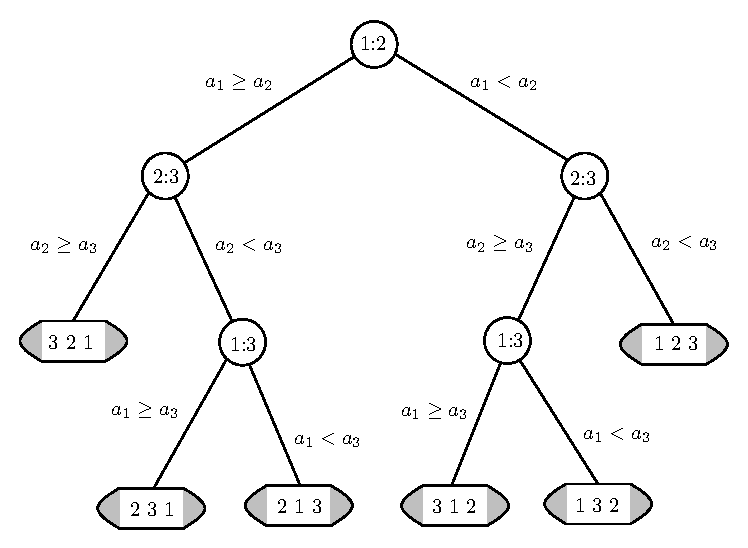
\includegraphics[width=80mm]{figs/tree123ipe.eps}
}
\caption{\label{tree123} Decision tree for $n=3$.}
\end{figure}

\begin{Example} A decision tree for three ($n=3$)
elements $a_1, a_2, a_3$ is shown in Figure~\ref{tree123}. 
Each internal tree node represents a pairwise comparison and decision made at a
particular step of sorting (in Figure~\ref{tree123}, $i:j$ denotes 
the comparison between the elements $a[i]$ and $a[j]$). 
Two downward arcs from the node indicate two possible
results of the comparison: $a[i] \geq a[j]$ or $a[i] < a[j]$. 
Leaves represent the sorted lists. In Figure~\ref{tree123}, each triple
$ijk$ denotes the sorted list $(a_i,a_j,a_k)$ obtained from
the initial list $(a_1 ,a_2 , a_3)$. For instance, \(123\),
\(213\), or \(321\) mean that the final list
is $(a_1 ,a_2 , a_3)$, $(a_2, a_1, a_3)$, or 
$(a_3 , a_2, a_1)$, respectively. 
Because any of the $n!$ permutations of $n$ arbitrary items 
$a_1, a_2, \ldots, a_n$ may be obtained as the result of 
the sort, the decision tree must have at least $n!$ leaves.
\end{Example}

The path length from the root to a leaf in the decision tree is equal to the 
number of comparisons  to be performed in order to  obtain the sorted array at 
the leaf. Therefore, the longest path (the height of the tree) equals
the number of comparisons in the worst case. For example, $3$ elements 
can be sorted with no more than $3$ comparisons because the height of the 
$3$-element tree in Figure~\ref{tree123} is equal to $3$. 

\begin{Theorem} \label{t:worst}
Every comparison-based sorting algorithm takes $\Omega(n\log n)$ time in the 
worst case.
\end{Theorem}

\begin{proof} 
We first claim that each binary tree of height $h$ has at most $2^{h}$ leaves. 
Once this claim is established, we proceed as follows. The least value $h$ such 
that $2^{h} \ge n!$ has the lower bound $h \ge \lg (n!)$ which is in
$\Omega(n \log n )$ (the asymptotic result follows from 
Section~\ref{sec:app:sum:series}). This will prove the theorem.

To prove the above claim about tree height, we use mathematical induction on 
$h$. A tree of height $0$ has obviously at most $2^{0}$ leaves. Now suppose 
that $h\geq 1$ and that each tree of height $h-1$ has at most $2^{h-1}$ 
leaves. The root of a decision tree of  height $h$ is linked to two subtrees, 
being each at most of height $h-1$. By the induction hypothesis, each 
subtree has at most $2^{h-1}$ leaves. The number of leaves in the whole decision
tree is equal to the total number of leaves in its subtrees, that is,
at most $2^{h-1}+2^{h-1}=2^{h}$.
\end{proof}

This result shows that heapsort and mergesort have asymptotically optimal 
worst-case time complexity for comparison-based sorting.

As for average-case complexity, one can also prove the following
theorem by using the decision tree idea. Since we are now at the end of
our introductory analysis of sorting, we omit the proof and refer the
reader to the exercises, and to more advanced books.

\begin{Theorem}\label{t:average}
Every comparison-based sorting algorithm takes $\Omega(n \log n)$ time
in the average case. 
\end{Theorem}

\begin{proof}
Try to prove this yourself (see Exercise~\ref{ex:prove-lower-bound}).
\end{proof}
\subsection*{Exercises}

\begin{Exercise} \label{ex:prove-lower-bound} 
Prove Theorem~\ref{t:average}. The following hints may be useful. First
show that the sum of all depths of leaves in a binary decision tree with $k$
leaves is at least $k \lg k$. Do this by  induction on $k$, using the
recursive structure of these trees. Then apply the above inequality 
with $k=n!$.
\end{Exercise}

\begin{Exercise}
\label{ex:radix}
Consider the following sorting method (often called \defnfont{counting sort}) 
applied to an array $a[n]$ all of whose entries are integers in the range 
$1..1000$. Introduce a new array $t[1000]$ all of whose entries are initially 
zero. Scan through the array $a[n]$ and each time an integer $i$ is found, 
increment the counter $t[i-1]$ by $1$. Once this is complete, loop through 
$0 \leq i\leq 999$ and print out $t[i]$ copies of integer $i+1$ at each step.

What is the worst-case time complexity of this algorithm? How do we reconcile 
this with Theorem~\ref{t:worst}?
\end{Exercise}


\section{Notes}
It was once said that sorting consumes 25\% of all CPU time worldwide. Whatever
the true proportion today, sorting clearly remains a fundamental problem to be 
solved in a wide variety of applications.

Given the rise of object-oriented programming languages,  comparison-based 
sorting algorithms are perhaps even more important than in the past. In practice
the time taken to perform a basic comparison operation is often much more than that 
taken to swap two objects: this differs from the case of, say, 32-bit integers,
for which most analysis was done in the past. 

Shellsort was proposed by D. Shell in 1959, quicksort by C. A. R. Hoare in 1960,
mergesort in 1945 by J. von Neumann, and heapsort in 1964 by J. W. J. Williams. 
Insertion sort and the other quadratic algorithms are very much older.

At the time of writing, versions of mergesort are used in the standard libraries for
the languages Python, C++ and Java, and a hybrid of quicksort and heapsort is used
by C++.

We have not discussed whether there is an algorithm that will find the 
median (or any other given order statistic) in worst-case linear time.
For a long time this was unknown, but the answer was shown to be yes in 1973 by 
Blum, Floyd, Pratt, Rivest and Tarjan. The algorithm is covered in more 
advanced books and is fairly complicated. 



